Raumlufttechnische Anlagen beinhalten unterschiedlichste Komponenten, beispielsweise Ventilatoren, Luftdrucksensoren und Temperatursensoren, mit denen die Funktion überwacht und gesteuert wird. Weil die \acs{rltanlagen} der Firma Bösch auf Kundenanforderungen angepasst werden, ist die Anordnung und Menge der verbauten Komponenten in den meisten Fällen unterschiedlich. Daher ist es wichtig, dass die \acs{rltanzeige} parametrierbar ausgeführt werden kann. Um dies zu erzielen, wurde vom Projektauftraggeber die Idee einer Konfigurationsdatei vorgeschlagen. Mit dieser kann von einer  Servicetechnikerin \bzw einem Servicetechniker bei der Installation der \acs{rltanlage} die Konfiguration an die \acs{rltanzeige} übergeben werden. So können für die jeweilige \acs{rltanlage} immer die richtigen Parameter angezeigt werden.

Wegen der Tatsache, dass diese Konfigurationsdateien von Servicetechnikerinnen und Servicetechnikern erstellt werden müssen, ist es wichtig, dass das gewählte Datenformat für Laien einfach zu verstehen ist. Daher lag die Entscheidung für das richtige Datenformat zwischen \acs{csv} und \acs{json}. Andere Formate  wie \acf{xml} wurden nicht in Erwägung gezogen, weil das Projektteam mit \acs{json} und \acs{csv} schon vertraut war. Darüber hinaus ist \acs{xml} im Vergleich zu \acs{json} für Laien schwerer zu lesen und schreiben, was es für die Anwendung ungeeignet macht. 

\subsection{Was ist \acs{csv}?}
\acf{csv} ist ein systemunabhängiges Format für Klartextdateien mit der Dateiendung \enquote{.csv}. \acs{csv} Dateien dienen zum Speichern und Übertragen von strukturierten Daten, hauptsächlich Tabellen oder Listen, wobei durch die Verkettung von mehreren \acs{csv} Dateien oder mithilfe von zusätzlichen Regeln auch verschachtelte Objekte gespeichert werden können. Die hauptsächlichen Anwendungsbereiche von \acs{csv} Dateien sind zum Importieren und Exportieren von Daten aus Datenbanken oder die Migration von Tabellendaten zwischen Programmen. \cite[vgl.][]{FuchsMediaSolutions:o.J.}

Die erste Verwendung des Datenformates geht auf 1972 zurück, wo es vom IBM FORTRAN IV (H Extended) Compiler unterstützt wurde. \cite[vgl.][]{IBM:1972} Trotz der langen Existenz gibt es gegenwärtig für \acs{csv} keine formelle Spezifikation. Mit dem \acs{rfc} 4180 \cite[vgl.][]{Shafranovich:2005} aus dem Jahre 2005 existiert ein erster Versuch einer inoffiziellen Definition, welche mittlerweile weit verbreitet ist. Durch dieses Dokument wird das \acf{mime} \enquote{text/csv} für das \acs{csv} Format registriert. Es folgen die wesentlichen Merkmale aus der Definition des \acs{rfc} 4180:

\begin{enumerate}{}
	
	\item Jedem Datensatz steht eine Zeile zu, die mit einem Zeilenumbruch (\ac{crlf}) beendet wird. Ein Zeilenumbruch am Ende des letzten Datensatzes ist optional. \zB 
	\begin{lstlisting}
	aaa, bbb, ccc CRLF
	xxx, yyy, zzz CRLF
	\end{lstlisting}
	oder
	\begin{lstlisting}
	aaa, bbb, ccc CRLF
	xxx, yyy, zzz
	\end{lstlisting}
	
	\item Am Anfang eines \acs{csv} Dokumentes kann es eine Kopfzeile geben. Diese hat das Format eines normalen Datensatzes und beinhaltet Namen für die Spalten (Felder). Die Anzahl der Spalten sollte für Kopfzeile und Datensätze gleich sein. \zB
	\begin{lstlisting}
	spaltenname_1, spaltenname_2, spaltenname_3 CRLF
	xxx, yyy, zzz CRLF
	\end{lstlisting} %	aaa, bbb, ccc CRLF
	
	\item Sowohl in den Datensätzen als auch in der Kopfzeile kann es eine oder mehrere Spalten geben, die jeweils immer durch einen Beistrich (\acs{engl} comma) separiert werden. Am Ende einer Zeile bedarf es keines Beistrichs. Abstände sind Teil eines Feldes und müssen berücksichtigt werden. (Anmerkung: Auch wenn das eigentliche Format Beistriche für die Feldtrennung vorsieht, werden oft andere Zeichen wie \zB Strichpunkte (Semikolons) verwendet.)
	
	\item Jedes Feld kann in Anführungszeichen eingeschlossen sein und darf dann auch Beistriche, Zeilenumbrüche oder Anführungszeichen beinhaltet. \zB
	\begin{lstlisting}
	"aaa","b CRLF
	bb","ccc" CRLF
	xxx,yyy,zzz
	\end{lstlisting}
	
\end{enumerate}

Da es bei \acs{csv} keine festen Vorgaben beim Datenformat gibt, ist es die Verantwortung der Benutzer sich auf eine Formatierung zu einigen. Das führt oft zu Problemen bei Zeit- und Datumsangaben oder bei der Verwendung von Sonderzeichen. Eine weitere Hürde ist die fehlende explizite Angabe des verwendeten Zeichensatzes, womit \zB Umlaute fehlerhaft dargestellt werden können. \cite[vgl.][]{FuchsMediaSolutions:o.J.}

\subsection{Was ist \acs{json}?}
\begin{minipage}{0.6\textwidth}
	\acf{json} wurde 2001 auf der \enquote{JSON.org} Website veröffentlicht und ist ein ressourcenschonendes Textformat zum Speichern von strukturierten Daten. Es ist so konzipiert, dass es sowohl für Menschen einfach zu lesen und schreiben als auch für Maschinen einfach zu parsen und generieren ist. Die Dateiendung von \acs{json} Dateien ist \enquote{.json}. \acs{json} stammt von JavaScript, ist aber programmiersprachenunabhängig und folgt vielen Konventionen der C-basierten Sprachen, was es gut für den Datenaustausch macht. \cite[vgl.][]{json_org:o.J., ECMA:2017}
\end{minipage}%
\hfill
\begin{minipage}{0.37\textwidth}
	\centering	
	
\includegraphics[width=0.58\textwidth]{JSON_logo}
	\captionof{figure}[JSON Logo]{\acs{json} Logo (Quelle:\\
		 \url{https://en.m.wikipedia.org/wiki/File:JSON_vector_logo.svg}) \label{fig:json_logo}}
\end{minipage}
\vspace{1ex}

\acs{json} wird derzeit von zwei Spezifikation definiert, ECMA-404 \cite[vgl.][]{ECMA:2017} und RFC 8259 \cite[vgl.][]{Bray:2017}. Dabei unterscheidet sich nur die Beschreibung des Formats, die \acs{json} Syntax beider Spezifikationen ist ident. Folgend wird sich auf die Beschreibung der offiziellen JSON.org Website \cite[vgl.][]{json_org:o.J.} und somit auf ECMA-404 \cite[vgl.][]{ECMA:2017} bezogen.

Die zwei wichtigsten Strukturen auf denen \acs{json} aufbaut sind Name/Wert (\engl Key/Value) Paare und geordnete Listen von Werten. Dabei unterstützt \acs{json} sehr verschachtelte Strukturen. Um diese darzustellen, werden in der Syntax folgende Zeichen benötigt:
\begin{itemize}
	 \item Beistriche \lstinline|,|
	 \item Doppelpunkte \lstinline|:|
	 \item Eckige Klammern \lstinline|[ ]|
	 \item Geschwungene Klammern \lstinline|{ }|
\end{itemize}


Mithilfe dieser Syntax, kann man in \acs{json} folgende Strukturen umsetzen:
\begin{itemize}
	\item \textbf{Values} (\dt Werte) sind, entweder vom Typ \enquote{object}, \enquote{string}, \enquote{array}, \enquote{number} oder haben den Wert \enquote{false}, \enquote{true}, oder \enquote{null} (siehe Abb.~\ref{fig:json_value}).
	\begin{figure}[H]
		\centering
		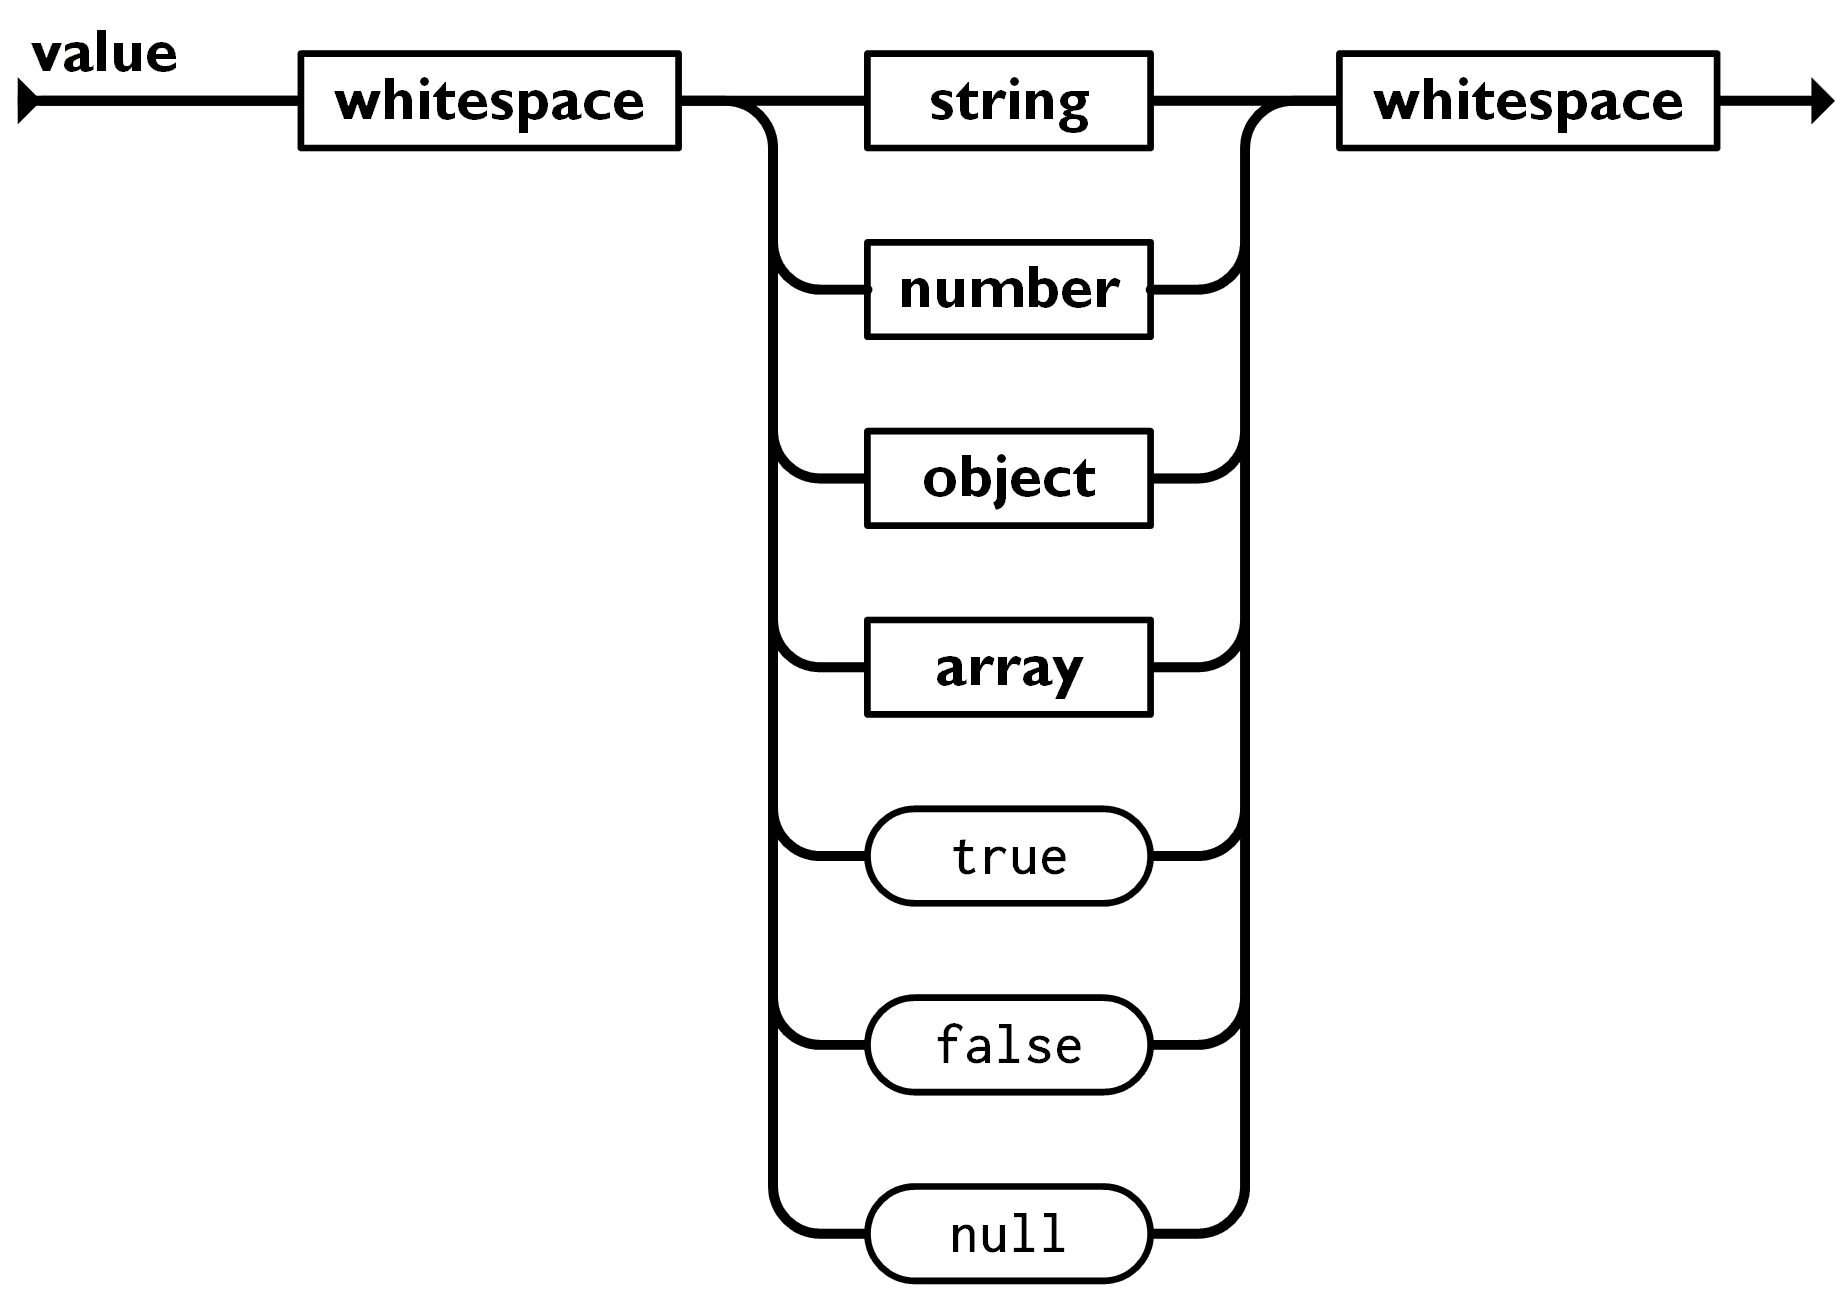
\includegraphics[width=10cm]{JSON_value}
		\caption[JSON Wert]{\acs{json} Value (Quelle: \url{https://www.json.org/img/value.png})  \label{fig:json_value}}
	\end{figure}
	
	\item \textbf{Objects} (\dt Objekte) sind ungeordnete Listen von beliebig vielen Name/Wert Paaren. Ein Name/Wert Paar besteht immer aus einem Namen, gefolgt von einem Doppelpunkt und dem zugehörigen Wert. Beistriche kommen zum Einsatz um Name/Wert Paare voneinander zu trennen. Ein Objekt wird immer von geschwungenen Klammern umschlossen. Der Aufbau eines \acs{json} Objekts ist in Abb.~\ref{fig:json_object} zu sehen.
	
	\begin{figure}[H]
		\centering
		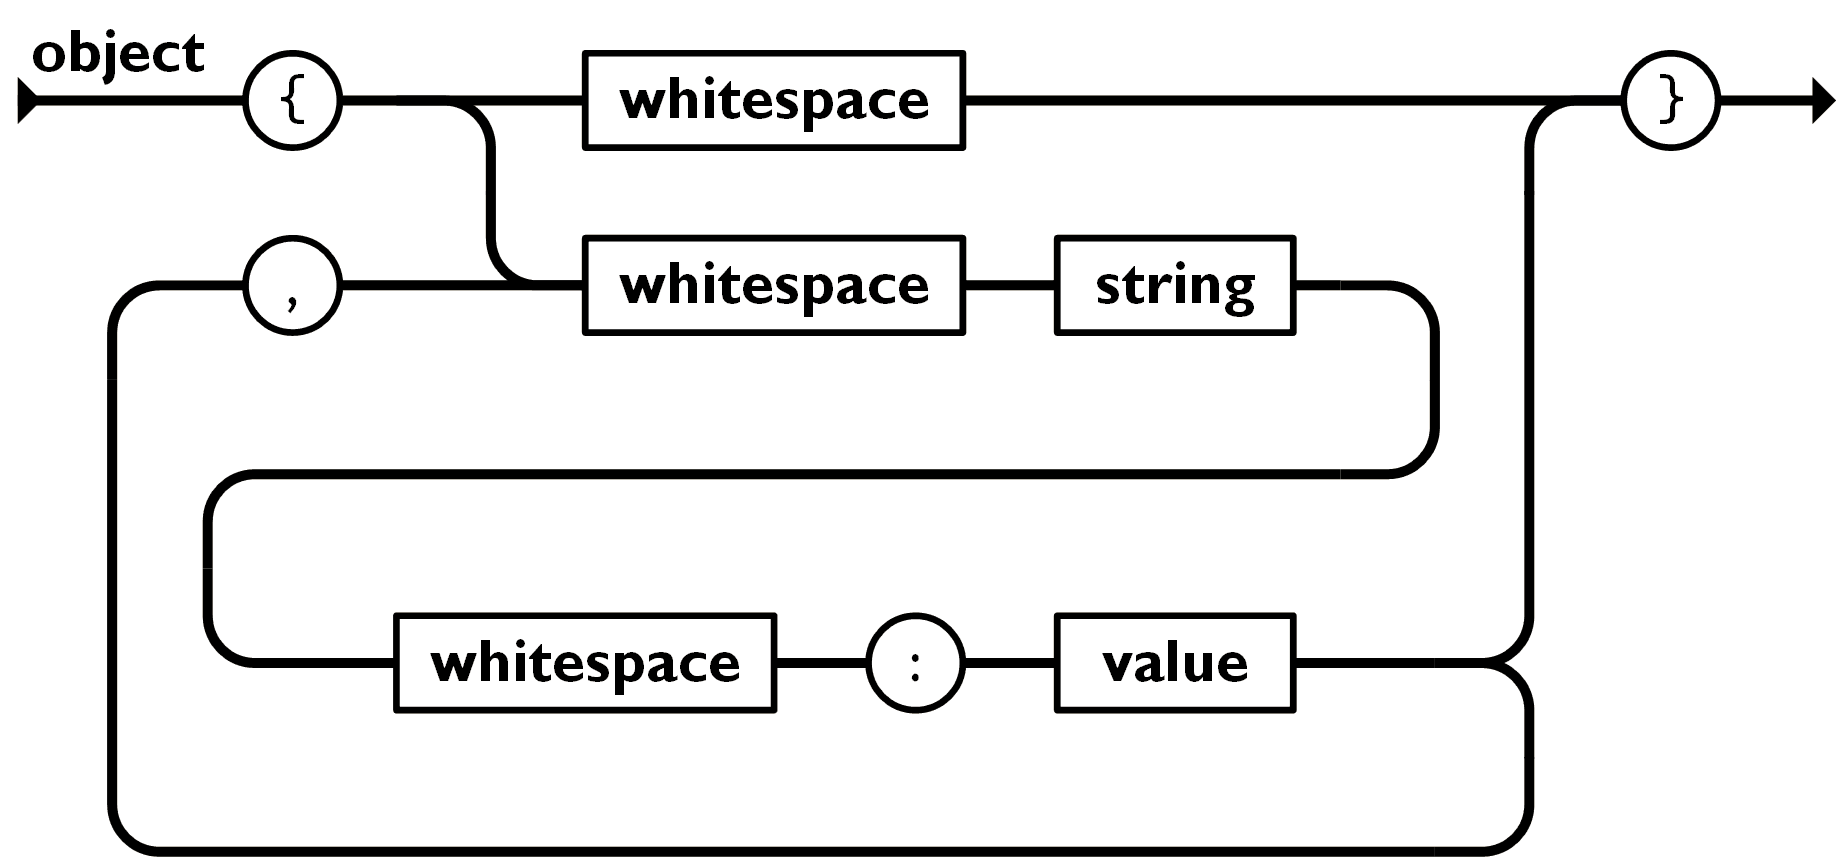
\includegraphics[width=10cm]{JSON_object}
		\caption[JSON Objekt]{\acs{json} Object (Quelle: \url{https://www.json.org/img/object.png})  \label{fig:json_object}}
	\end{figure}
	
	\item \textbf{Arrays} sind geordnete Listen von Werten. Dabei werden Beistriche verwendet, um die Werte voneinander zu trennen. Ein Array wird immer von eckigen Klammern umschlossen. Der Aufbau eines Arrays ist in Abb.~\ref{fig:json_array} zu sehen.
	
	\begin{figure}[H]
		\centering
		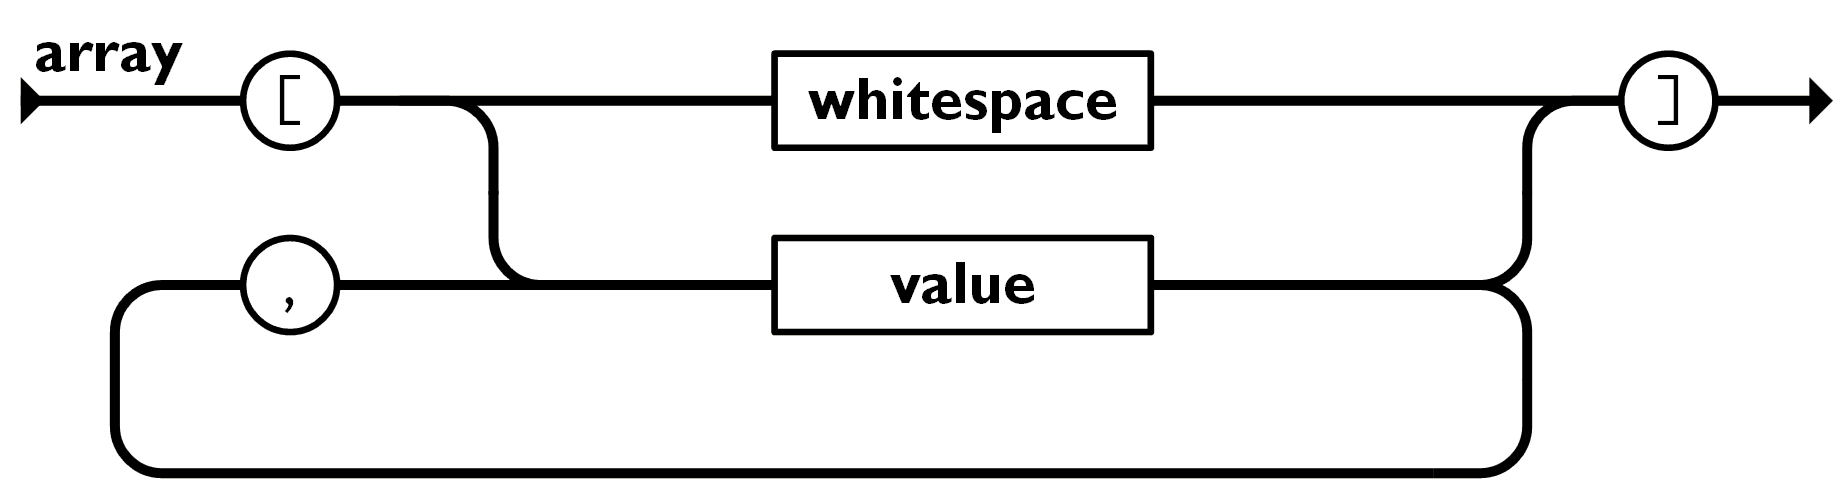
\includegraphics[width=10cm]{JSON_array}
		\caption[JSON Array]{\acs{json} Array (Quelle: \url{https://www.json.org/img/array.png})  \label{fig:json_array}}
	\end{figure}
	
	\item \textbf{Strings} sind Zeichenketten. Sie können entweder leer sein, d. h. aus keinen Zeichen bestehen oder mehrere Unicode Zeichen enthalten. Eine Zeichenkette wird immer von Anführungszeichen umschlossen. Sie kann auch besondere Escapesequenzen beinhalten, die besondere Bedeutungen haben. Diese werden mit einem Backslash aufgerufen, wie \zB \enquote{\textbackslash n}, \enquote{\textbackslash t} oder \enquote{\textbackslash r}.
	
	\item \textbf{Numbers} (\dt Zahlen) sind numerische Werte, die aus einer oder mehreren dezimalen Ziffern bestehen. Sie können also keine Werte wie \zB \enquote{Infinity} oder \enquote{NaN} annehmen. Außerdem werden sie nie von Anführungszeichen umschlossen. 
	
\end{itemize}

Beispiele für \acs{json} Dateien sind in Kapitel \ref{json_config_files} zu finden.

\subsection{\acs{json} und \acs{csv} - Vergleich und Selektion} \label{json_vs_csv}
Sowohl \acs{json} als auch \acs{csv} bringen Vorteile mit sich. 
\acs{csv} Dateien können in Microsoft Excel bearbeitet und erstellt werden. Die tabellarische Darstellung und die Bekanntheit von Excel machen es zugänglich für Laien, was der größte Vorteil für \acs{csv} ist. Außerdem wird \acs{csv} von vielen Programmiersprachen unterstützt, was die Umsetzung theoretisch möglich machen würde. 

\acs{json} Dateien sind hingegen \acs{csv} zwar für Laien schwererer zu lesen, bieten aber hinsichtlich meist anderer Aspekte deutlich mehr Möglichkeiten. Anstatt des tabellarischen Aufbaus wird zum Speichern der Daten eine klare hierarchische Struktur verwendet. Die Struktur sorgt für mehr Flexibilität und eine besonders gute Darstellung verschachtelter Daten. Auch unterstützt \acs{json} unterschiedliche Datentypen, während bei \acs{csv} grundsätzlich nur Zeichenketten zum Einsatz kommen.

\acs{json} ist mittlerweile an Kompatibilität kaum zu übertreffen, was dessen Verwendung unbedenklich macht. Das Datenformat wird in unzähligen Bereichen eingesetzt und der Trend scheint immer weiter gegen \acs{json} zu gehen.

Schließlich überwiegen, im benötigten Anwendungsbereich, die vielen Vorteile von \acs{json} die schlechtere Leserlichkeit. Vor allem war die Möglichkeit der Verschachtelung der ausschlaggebende Grund weshalb sich für das \acs{json} Datenformat entschieden wurde. Dazu ist es wahrscheinlich, dass, wegen ihrem logischen Aufbau und  Skalierbarkeit, \acs{json} Dateien für den Anwendungszweck im Endeffekt übersichtlicher als \acs{csv} Dateien sind.

Falls bei Einführung der \acs{rltanzeige} Schwierigkeiten mit der Konfiguration auftreten steht \zB die Option eines Skripts, welches Excel Dateien in das gewünschte \acs{json} Format übersetzt, zur Verfügung.

